\documentclass[cyan]{elegantnote}
\author{Yuyang Songsheng}
\email{songshengyuyang@gmail.com}
\zhtitle{物理}
\entitle{Physics}
\version{1.00}
\myquote{Summary is the best way to say "Good Bye"}
\logo{logo.jpg}
\cover{cover.pdf}
%green color
   \definecolor{main1}{RGB}{210,168,75}
   \definecolor{seco1}{RGB}{9,80,3}
   \definecolor{thid1}{RGB}{0,175,152}
%cyan color
   \definecolor{main2}{RGB}{239,126,30}
   \definecolor{seco2}{RGB}{0,175,152}
   \definecolor{thid2}{RGB}{236,74,53}
%cyan color
   \definecolor{main3}{RGB}{127,191,51}
   \definecolor{seco3}{RGB}{0,145,215}
   \definecolor{thid3}{RGB}{180,27,131}

\usepackage{mhchem}
\usepackage{makecell}
\usepackage{lipsum}
\usepackage{amssymb}
\usepackage{float}
\usepackage{wrapfig}
\usepackage{latexsym}
\usepackage{hyperref}
\usepackage{feynmf}
\usepackage{exscale}
\usepackage{relsize}
\usepackage{slashed}
\usepackage{mathrsfs}
\usepackage{bm}%bold math, for vector


\begin{document}
\maketitle
\tableofcontents
\newpage
\section{Linear sigma model}
\subsection{Introduction}
\[\mathcal{L} = -\frac{1}{2} \partial_{\mu} \phi^i \partial^{\mu}\phi^i + \frac{1}{2} \mu^2 (\phi^i)^2 - \frac{\lambda}{4} [(\phi^i)^2]^2\]
The Lagrangian is invariant under the symmetry
\[\phi^i \to R^{ij} \phi^j\]
for any $N \times N$ orthogonal group in $N$ dimensions, also called the $N$-dimensional orthogonal group or simply $O(N)$. In classical theory, the lowest-energy classical configuration is a constant field $\phi_0^i$, whose value is chosen to minimize the potential
\[V = -\frac{1}{2}\mu^2 (\phi^i)^2 + \frac{\lambda}{4}[(\phi^i)^2]^2\]
This potential is minimized for any $\phi_0^i$ that satisfies
\[(\phi^i)^2 = \frac{\mu^2}{\lambda} \]
This condition determines only the length of the vector $\phi_0^i$, its direction is arbitrary. 
It is conventional to choose coordinates so that $\phi_0^i$ points in the $N$th direction
\[\phi_0^i = (0,0,\cdots,0,v) \quad v \equiv \frac{\mu}{\sqrt{\lambda}}\]
We can now define a set of shifted fields by writing
\[\phi^i = (\pi^k,v+\sigma) \quad k = 1,\cdots,N-1\]
It is now straightforward to rewrite the Lagrangian in terms of the $\pi$ and $\sigma$ fields. The result is
\begin{eqnarray}
\mathcal{L} &=& -\frac{1}{2}(\partial_{\mu}\pi^k)^2 - \frac{1}{2}(\partial_{\mu}\sigma)^2 - \frac{1}{2}(2\mu^2)\sigma^2 \nonumber \\
&-& \sqrt{\lambda}\mu \sigma^3 - -\sqrt{\lambda}\mu (\pi^k)^2\sigma - \frac{\lambda}{4}\sigma^4 - \frac{\lambda}{2}(\pi^k)^2\sigma^2 - \frac{\lambda}{4}[(\pi^k)^2]^2 \nonumber
\end{eqnarray}
We obtain a massive $\sigma$ field and also a set of $N-1$ massless $\pi$ fields. The original $O(N)$ symmetry is hidden when we choose a specific $\phi_0^i$ for vacuum state, leaving only the subgroup $O(N-1)$, which rotates the $\pi$ fields among themselves. Given the Goldstone's theorem, our discussion here will remain valid when quantum correction is considered.

\subsection{Renormalization}
From this expression of the Lagrangian written in terms of shifted fields, we can read off the Feynman rules for the linear sigma model. Then we can compute tree-level amplitudes without difficulty.
\\
\begin{figure}[!h]
\centering
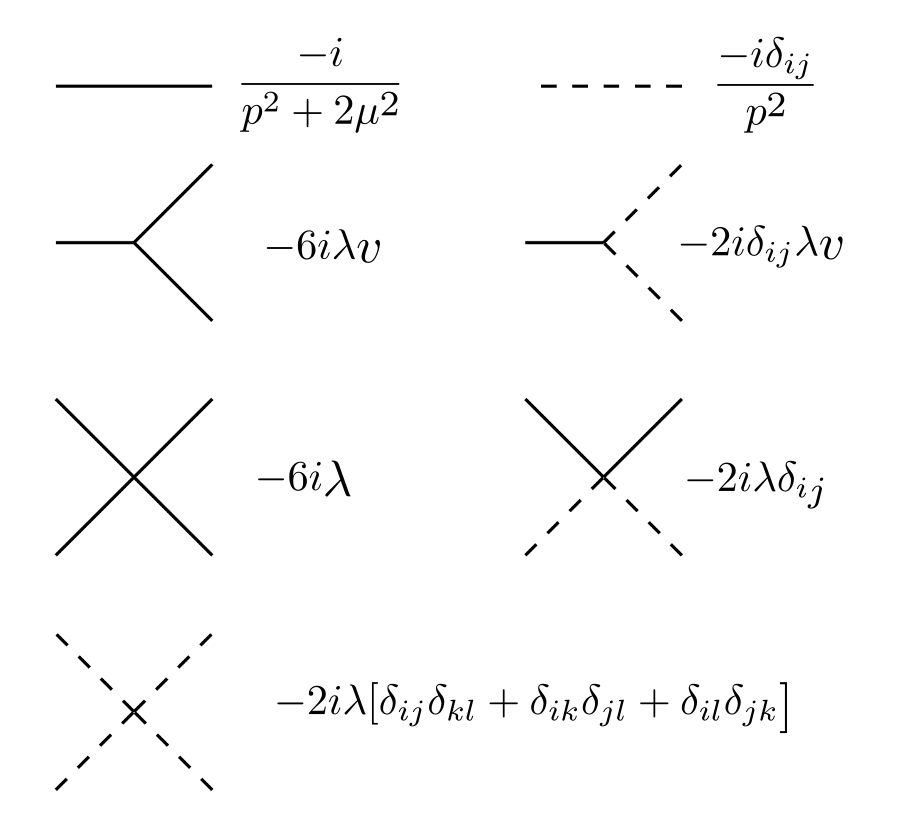
\includegraphics[scale=0.2]{QFT1/Li_sigma1.png}
\caption{Feynman rules for the linear sigma model}
\end{figure}
\\
Diagrams with loops, however, will often diverge. For the amplitude with $N_e$ external legs, the superficial degree of divergence is
\[D = 4 - N_e\]
The linear sigma model has eight different superficially divergent amplitudes and several of these have $D > 0$ and therefore can contain more than one infinite constant.
\\
\begin{figure}[!h]
\centering
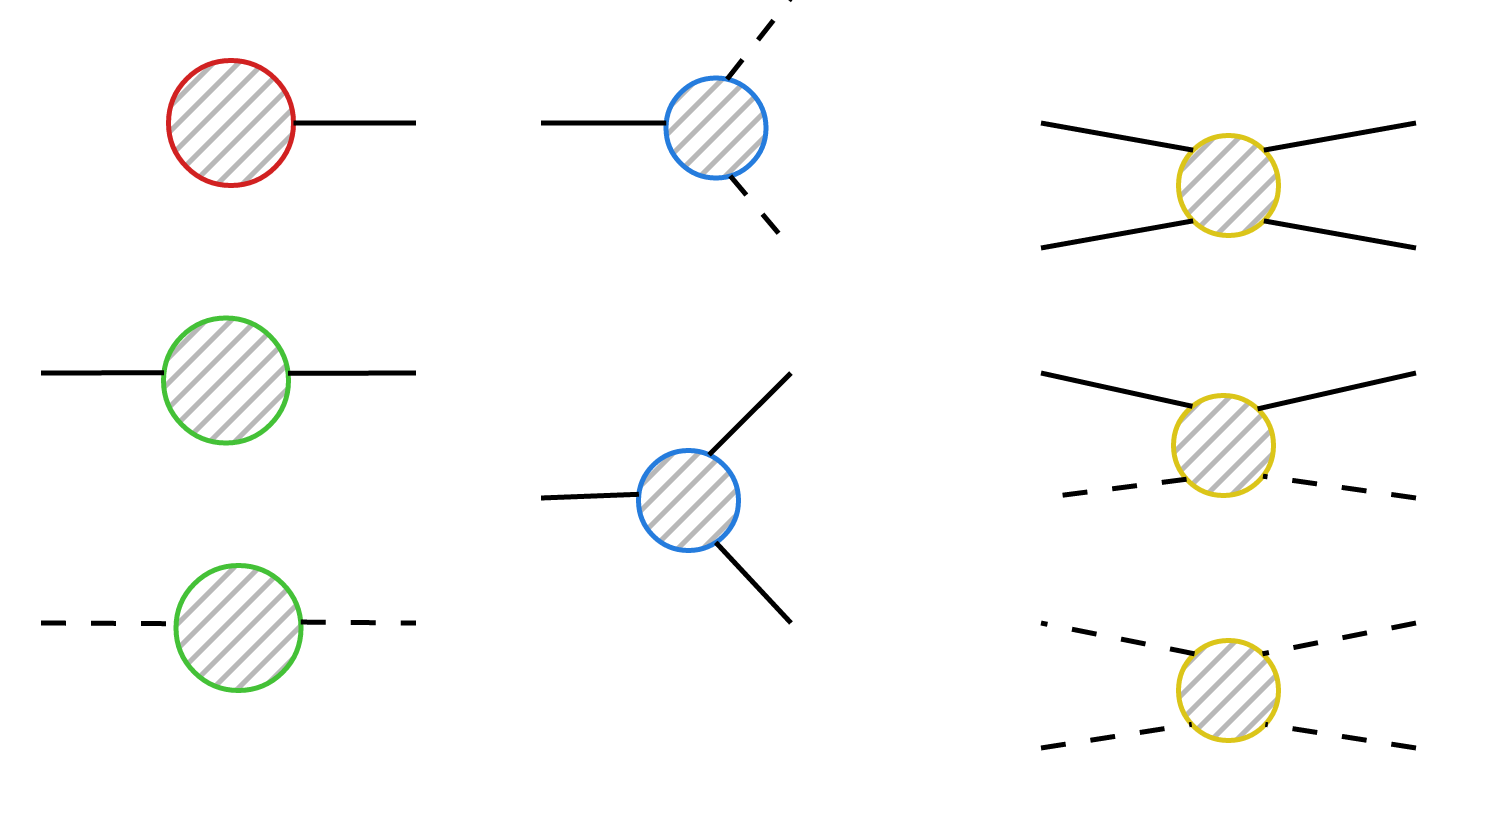
\includegraphics[scale=0.2]{QFT1/Li_sigma2.png}
\caption{Divergent amplitudes in the linear sigma model}
\end{figure}
\\
Yet we have only three counterterms:
\[\mathcal{L}_{ct} = -\frac{1}{2} \delta_Z \partial_{\mu} \phi^i \partial^{\mu}\phi^i - \frac{1}{2} \delta_{\mu} (\phi^i)^2 - \frac{\delta_{\lambda}}{4} [(\phi^i)^2]^2 \]
Written in terms of $\sigma$ and $\pi$ fields, we have
\begin{eqnarray}
\mathcal{L}_{ct} &=& -\frac{\delta_Z}{2}(\partial_{\mu}\pi^k)^2 - \frac{1}{2}(\delta_{\mu}+\delta_{\lambda}v^2)(\pi^k)^2 -\frac{\delta_Z}{2}(\partial_{\mu}\sigma)^2 - \frac{1}{2}(\delta_{\mu} + 3\delta_{\lambda}v^2)\sigma^2 \nonumber \\
&-& (\delta_{\mu}v + \delta_{\lambda}v^3)\sigma - \delta_{\lambda}v\sigma(\pi^k)^2 - \delta_{\lambda}v\sigma^3 - \frac{\delta_{\lambda}}{4}[(\pi^k)^2]^2 - \frac{\delta_{\lambda}}{2}\sigma^2 (\pi^k)^2 - \frac{\delta_{\lambda}}{4}\sigma^4 \nonumber
\end{eqnarray}
We can get the Feynman rules associated with these counterterms.
\\
\begin{figure}[!h]
\centering
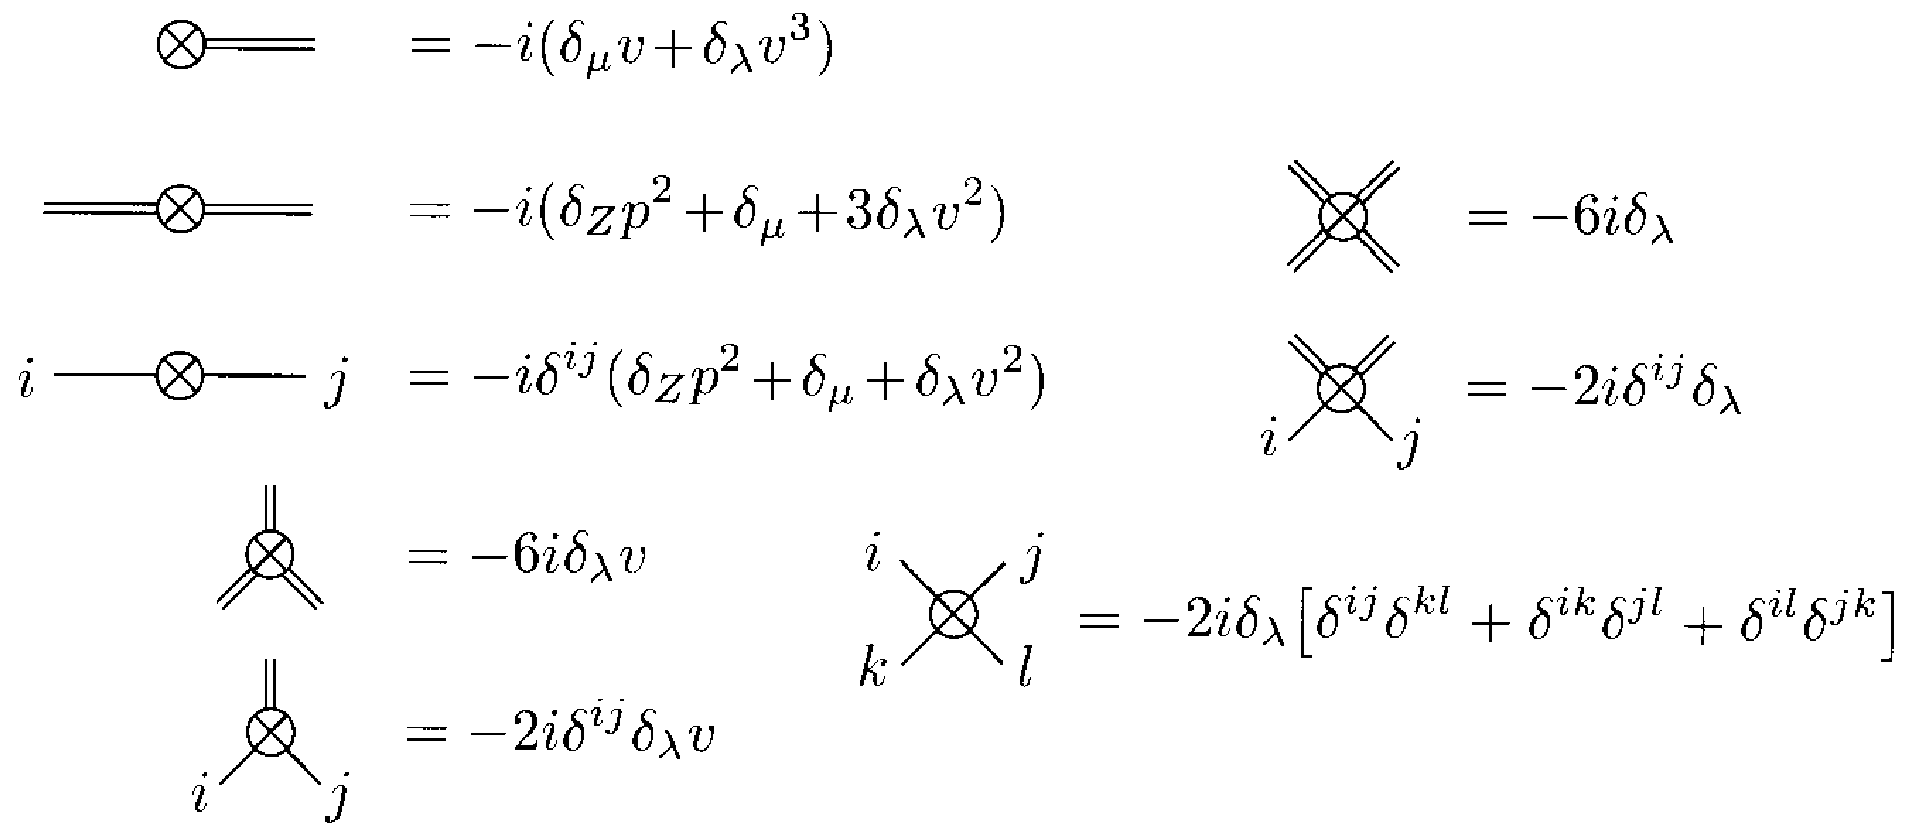
\includegraphics[height=5cm ,width=11.46cm]{QFT1/Li_sigma3.png}
\caption{Feynman rules for counterterm vertices in the linear sigma model}
\end{figure}
\\
We can also set renormalization conditions for linear sigma model.
\begin{figure}[!h]
\centering
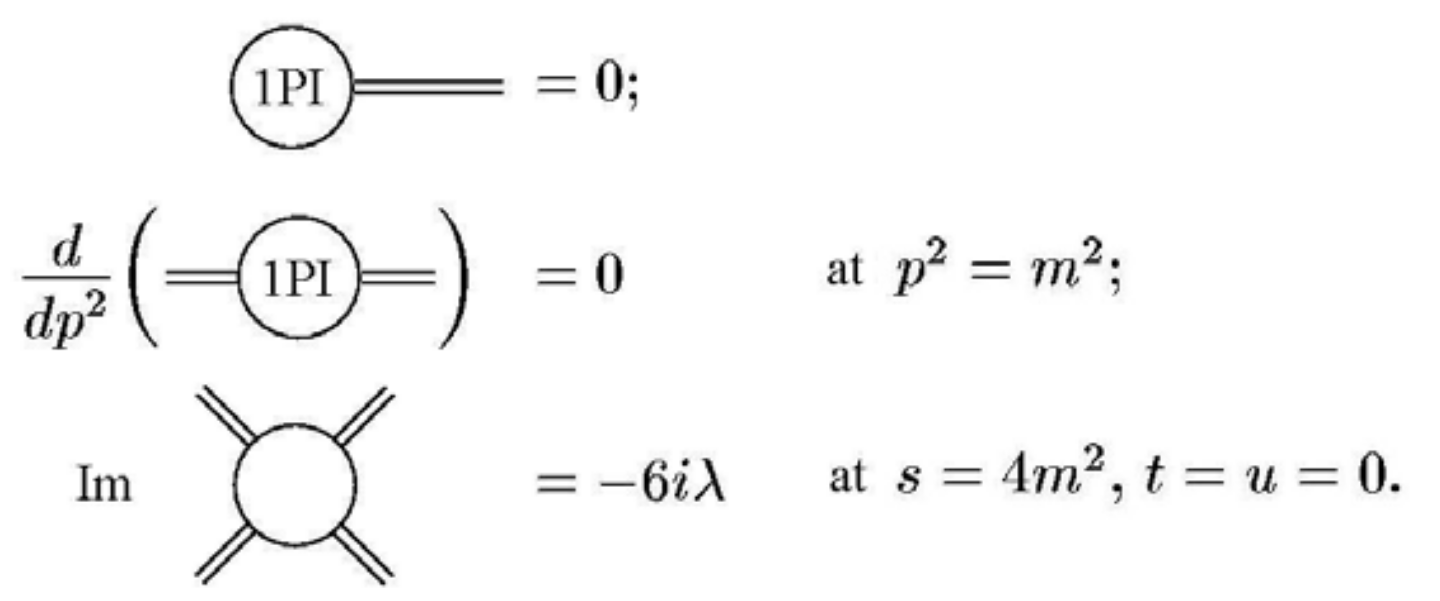
\includegraphics[height=3cm ,width=7.2cm]{QFT1/Li_sigma4.png}
\caption{Renormalization conditions ($m^2 = 2\mu^2$)}
\end{figure}
\\
One-loop corrections for linear sigma model has been calculated in section 11.2 of \emph{An introduction to quantum field theory (M.E.Peskin \& D.V.Schroeder)}. There are two important results.
\begin{itemize}
\item All the divergence up to one loop will be cancelled by adjusting three counterterms. Apparently, the divergent part of the diagram is unaffected by the symmetry breaking.
\item The propagator of $\pi\pi$ has a pole at $p^2 = 0$ after one loop correction, i.e. $\pi$ particles remain massless after one loop correction.
\end{itemize}

\subsection{Effective action}
We begin again with the Lagrangian
\[\mathcal{L}_1 = -\frac{1}{2} \partial_{\mu} \phi^i \partial^{\mu}\phi^i + \frac{1}{2} \mu^2 (\phi^i)^2 - \frac{\lambda}{4} [(\phi^i)^2]^2\]
Expand about the classical field $\phi^i = \phi_{\mathrm{cl}}^i + \eta^i$, and we assume the vacuum is translational invariant. Then we have
\[\mathcal{L}_1 = -\frac{1}{2}(\partial_{\mu}\eta)^2 + \frac{1}{2}\mu^2(\eta^i)^2 - \frac{\lambda}{2}[(\phi_{\mathrm{cl}}^2)(\eta^i)^2+ 2(\phi_{\mathrm{cl}}^i\eta^i)^2] + \cdots\]
From the terms quadratic in $\eta$, we can read off
\[\frac{\delta^2 \mathcal{L}_1}{\delta\phi^i\delta\phi^j} = \partial^2\delta_{ij} + \mu^2\delta_{ij} - \lambda[(\phi_{\mathrm{cl}}^k)^2\delta_{ij} + 2\phi_{\mathrm{cl}}^i \phi_{\mathrm{cl}}^j]\]
We choose the vacuum state by demanding $\phi_{\mathrm{cl}}^i$ points in the $N$th direction
\[\phi_{\mathrm{cl}}^i = (0,\cdots,\phi_{\mathrm{cl}})\]
Then the operator is just equal to the Klein-Gordon operator $(\partial^2-m_i^2)$, where
\[m_i^2 = \begin{cases} \lambda\phi_{\mathrm{cl}}^2-\mu^2 \quad i=1,\cdots,N-1 \\ 3\lambda\phi_{\mathrm{cl}}^2-\mu^2 \quad i=N \end{cases}\]
We would perform the calculation of $\log Z_0[0]$ in the next subsection. Here, we just list the result:
\[\log Z_0[0] = \frac{i}{2}\frac{\Gamma(-\frac{d}{2})}{(4\pi)^{d/2}}(m^2)^{\frac{d}{2}}VT\]
So, up to one loop corrections, we can get
\[V_{\mathrm{eff}} = -\frac{1}{2} \mu^2 \phi_{\mathrm{cl}}^2 + \frac{\lambda}{4} \phi_{\mathrm{cl}}^4 - \frac{1}{2}\frac{\Gamma(-\frac{d}{2})}{(4\pi)^{d/2}}[(N-1)(\lambda\phi_{\mathrm{cl}}^2-\mu^2)^{\frac{d}{2}} + (3\lambda\phi_{\mathrm{cl}}^2-\mu^2)^{\frac{d}{2}}] + \frac{1}{2}\delta_{\mu}\phi_{\mathrm{cl}}^2 + \frac{1}{4}\delta_{\lambda}\phi_{\mathrm{cl}}^4\]
And if we want $V_{\mathrm{eff}}$ is finite for terms involving $\phi_{\mathrm{cl}}$, we can get
\[\delta_{\lambda} = \frac{2\lambda^2(N+8)}{(4\pi)^2} \times \frac{1}{4-d} + \mbox{ finite terms }\]
\[\delta_{\mu} = -\frac{2\lambda\mu^2(N+2)}{(4\pi)^2} \times \frac{1}{4-d} + \mbox{ finite terms }\]
It is the same result as that in previous section.

\subsection{Functional determinants}
\[Z_0[0] \equiv \prod_{i=1}^{N} Z_i  = \prod_{i=1}^{N} \int \mathcal{D}\eta e^{ \frac{i}{2}\int \eta \left( \partial^2-m_i^2\right) \eta }\]
Here, $m_i$ is a function of $\phi_{cl}$. We want to get $\log Z_0[0]$ as a function of $\phi_{cl}$ and the  infinite constant shift of $\log Z_0[0]$ will be dropped . We treat $-\frac{1}{2}m_i^2\eta^2$ as a perturbation, so we have
\[Z_i \propto e^{-\frac{im_i^2}{2}(\frac{1}{i} \frac{\delta}{\delta I})^2} \left. \int \mathcal{D}\eta e^{i\int \left(-\frac{1}{2} I D_F I \right)} \right|_{I=0}\] 
where
\[D_F(x-y) = \int \frac{d^4p}{(2\pi)^4} \frac{-i}{p^2}e^{ip(x-y)}\]
Now we can have the following Feynamn rules.
\begin{itemize}
\item A line from $x$ to $y$ is associated with $D_F(x-y)$
\item A vertex joining two lines at $x$ is associated with $-im_i^2\int d^4x$
\end{itemize}
So we have
\[\log Z_i = \sum_{I}C_I\]
where $C_I$ represents connected diagram without external source.
\\
\begin{figure}[!h]
\centering
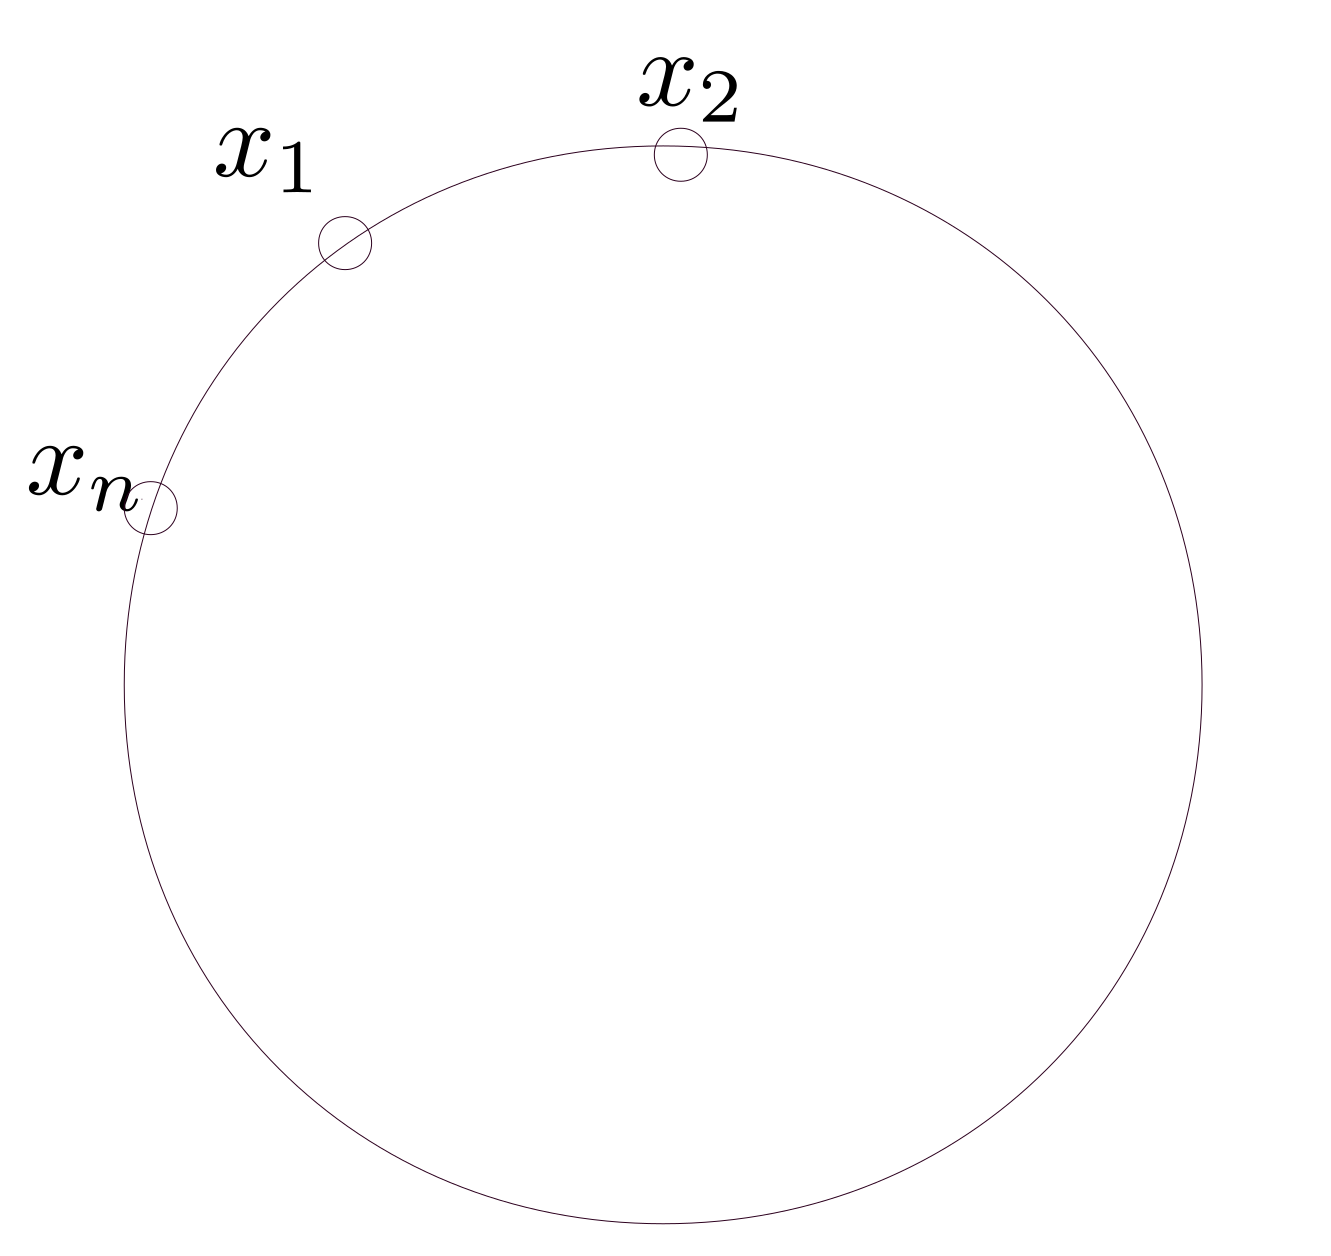
\includegraphics[scale=0.15]{QFT1/effective.png}
\caption{Connected Feymann diagram without external source}
\end{figure}
\\
So, we have
\[C_n = \frac{1}{2n}\int \prod_{k=1}^{n} \frac{d^4p_k d^4x_k}{(2\pi)^4} \frac{-m_i^2}{p_k^2} \exp(ip_k(x_k-x_{k+1})) = \frac{1}{2n} \int d^4p \delta(0) \left(-\frac{m_i^2}{p^2} \right)^n\] 
\[\log Z_i = -\frac{1}{2}VT \int \frac{d^4p}{(2\pi)^4} \sum -\frac{1}{n} \left(-\frac{m_i^2}{p^2} \right)^n = -\frac{1}{2}VT\int  \frac{d^4p}{(2\pi)^4} \log(1+\frac{m_i^2}{p^2})\]
The following calculation needs tricks of wick rotation and dimension regularization and you can refer to the equation 11.72 of \emph{An introduction to quantum field theory (M.E.Peskin \& D.V.Schroeder)}.
\\ \\
However, recall the Gaussian integral
\[\int _{-\infty }^{\infty }e^{\left(-{\frac {i}{2}}\sum \limits _{i,j=1}^{n}A_{ij}x_{i}x_{j}\right)}\,d^{n}x
= {\sqrt {\frac {(-2\pi i)^{n}}{\det A}}} \]
So formally, we have
\[\log Z_i = -\frac{1}{2}\log \det (-\partial_x^2 + m_i^2)\delta(x-y)\]
Define
\[M(x-y) \equiv (-\partial_x^2 + m_i^2)\delta(x-y) \quad M_0(x,y) \equiv -\partial_x^2\delta(x-y) \quad M_1(y,z) \equiv \delta(y-z) + im_i^2D_F(y-z)\]
We can verify that
\[M(x,z) = \int d^4y M_0(x-y)M_1(y-z)\]
So, 
\[\log \det M = \log \det M_0 + \log \det M_1 \to \log \det M_1\]
We drop out $\log \det M_0$ because it does not contain $m(\phi_{\mathrm{cl}})$. Furthermore, we have $M_1 = I - G$, where $I = \delta(x-y)$ is the identity matrix and $G = -im_i^2D_F$. So
\[\log \det M_1 =  \mathrm{Tr} \log M_1 = \mathrm{Tr} \log(I-G) = -\frac{1}{n}\sum_{n=1}^{\infty} \mathrm{Tr} G^n\]
We can verify that
\[C_n = \frac{1}{2n} \mathrm{Tr} G^n\]
So, the function determinant method is valid.

\section{Optical theorem and unstable particles}
The optical theorem is a straightforward consequence of the unitarity of the $S$ -matrix: $S^{\dagger}S = 1$. 
Inserting $S = 1 + iT$, we have
\[-i(T - T^{\dagger}) = T^{\dagger}T\]
Recall that
\[\langle f | iT | i \rangle = i\mathcal{M}(2\pi)^4\delta(\sum p_f - \sum p_i)\]
We have
\[\langle f | T^{\dagger}T | i \rangle = \sum_n \prod_{k=1}^n \int \frac{d^3q_k}{(2\pi)^3 2E_k} \langle f | T^{\dagger} | \{\bm{q}_k\} \rangle \langle \{\bm{q}_k\} | T | i \rangle\]
So, we have
\[-i[\mathcal{M}(i \to f) - \mathcal{M}^{*}(f \to i)] =  \sum_n \prod_{k=1}^n \int \frac{d^3q_k}{(2\pi)^3 2E_k} \mathcal{M}(i \to \{\bm{q}_k\}) \mathcal{M}^{*}(f \to \{\bm{q}_k\}) (2\pi)^4 \delta(\sum p_f- \sum_k q_k)\]
Let us abbreviate this identity as
\[-i[\mathcal{M}(i \to f) - \mathcal{M}^{*}(f \to i)] = \sum_m \int d\Pi_{m} \mathcal{M}(i \to m) \mathcal{M}^{*}(f \to m)\]
where the sum runs over all possible sets of particles and $i$ and $f$ could be one-particle or multi-particle asymptotic states.
\\
If $i$ and $f$ are the same state, we have
\[\mathrm{Im} \mathcal{M}(i \to i) = \sum_m \int d\Pi_{m} |\mathcal{M}(i \to \mbox{ anything })|^2\]
Particularly, if $i$ is a two particle state, we have
\[\mathrm{Im} \mathcal{M}(k_1k_2 \to k_1k_2) = 2E_{\mathrm{cm}}p_{\mathrm{cm}}\sigma_{\mathrm{tot}}(k_1k_2 \to \mbox{ anything })\]
If $i$ is a one particle state, we have
\[\mathrm{Im} \mathcal{M}(k \to k) = 2E_{k}\Gamma_{\mathrm{tot}}(k \to \mbox{ anything })\]
It can be represented in terms of 1PI propagator as
\[\mathrm{Im} M^2(k^2) = -2E_{k}\Gamma_{\mathrm{tot}}(k \to \mbox{ anything })\]
\\
Consider a theory of two real scalar fields, $\phi$ and $\chi$, with Lagrangian
\[\mathcal{L} = -\frac{1}{2}\partial_{\mu}\phi \partial^{\mu}\phi - \frac{1}{2}m_{\phi}^2\phi^2 -\frac{1}{2}\partial_{\mu}\chi \partial^{\mu}\chi - \frac{1}{2}m_{\chi}^2\chi^2 + \frac{1}{2}g\phi\chi^2 + \frac{1}{6}h\phi^3\]
This theory is renormalizable in six dimensions, where $g$ and $h$ are dimensionless coupling constants. Let us assume that $m_{\phi} > 2m_{\chi}$ . Then it is kinematically possible for a $\phi$ particle at rest to decay into two $\chi$ particles.
The amplitude for this process is given at one loop level as
\[\Gamma = \frac{1}{2} \frac{1}{2m_{\phi}} \int d\Pi_m |\mathcal{M}|^2 = \frac{1}{12} \pi \alpha (1 - 4m_{\chi}^2/m_{\phi}^2)^{3/2}m_{\phi}\]
where $\alpha = g^2/(4\pi)^3$.
Note that the extra factor $1/2$ is due to the presence of two identical particles in the final state.
\\
Let us, then, compute the correction to the $\phi$ propagator from a loop of $\chi$ particles. (There is also a contribution from a loop of $\phi$ particles, but we can ignore it if we assume that $h \ll g$.) We have
\[M^2(k^2) = -\frac{1}{2}\alpha \int_0^1 dx D\ln D + A'k^2 + B'm_{\phi}^2\]
where
\[D = x(1-x)k^2 + m_{\chi}^2 - i\epsilon\]
and $A'$ and $B'$ are the finite counterterm coefficients that remain after the infinities have been absorbed. 
We now try to fix $A'$ and $B'$ by imposing the usual on-shell conditions $M^2(-m_{\phi}^2) = 0$ and $d M^2 / d(k^2)|_{k^2=-m_{\phi}^2} = 0$.
\\
But, we have a problem. For $k^2 = -m_{\phi}^2$ and $m_{\phi} > 2m_{\chi}$, $D$ is negative for part of the range of $x$. Therefore $\ln D$ has an imaginary part. 
This imaginary part cannot be cancelled by $A'$ and $B'$, since $A'$ and $B'$ must be real: they are coefficients of hermitian operators in the Lagrangian. 
The best we can do is $\mathrm{Re}[M^2(-m_{\phi}^2)] = 0$ and $\mathrm{Re}[(M^2)'(-m_{\phi}^2)] = 0$. Imposing these gives
\[M^2(k^2) = -\frac{1}{12}\alpha \int_0^1 dx \ln(D/|D_0|) + \frac{1}{12}\alpha(m_{\phi}^2 + k^2)\]
where
\[D_0 = -x(1-x)m_{\phi}^2 + m_{\chi}^2\]
Now let us compute the imaginary part of $M^2$. 
This arises from the integration range $x_- < x < x_+$, where $x_{\pm}$ are the roots of $D = 0$ when $k^2 < -4m_{\chi}^2$. 
In this range, $\mathrm{Im} \ln D = -i \pi$; the minus sign
arises because $D$ has a small negative imaginary part. Finally, we have
\[\mathrm{Im} M^2(-m_{\phi}^2) = -m_{\phi} \Gamma\]
To get a more physical understanding of this result, recall that in non-relativistic quantum mechanics, a metastable state with energy $E_0$ and angular momentum quantum number $l$ shows up as a resonance in the partial-wave scattering amplitude,
\[f_l \sim \frac{1}{E - E_0 + i\Gamma/2}\]
If we imagine convolving this amplitude with a wave packet $\tilde{\psi}(E)e^{-iEt}$ will find a time dependence
\[\psi(t) \sim \int dE \frac{1}{E-E_0+i\Gamma/2} \tilde{\psi}(E)e^{-iEt} \sim e^{-iE_0 t - \Gamma t /2}\]
Therefore $|\psi(t)|^2 \sim e^{-\Gamma t}$, and we identify $\Gamma$ as the inverse lifetime of the metastable state.

\section{Non-relativistic limit}
\subsection{Complex Klein-Gordon field}
The Lagrangian of complex Klein-Gordon field is
\[\mathcal{L} = - \partial^{\mu}\Phi^{\dagger}\partial_{\mu}\Phi - m^2\Phi^{\dagger}\Phi\]
The canonical momentum is
\[\pi = \dot{\Phi}^{\dagger} \quad \pi^{\dagger} = \dot{\Phi}\]
The commutation relations are
\[[\phi(\bm{x},t),\pi(\bm{y},t)] = i\delta(\bm{x}-\bm{y})\]
Since the equation of motion is
\[(\partial^2-m^2)\Phi = 0\]
we have the Fourier expansion
\[\Phi = \int \widetilde{dp} [b(\bm{p})e^{ipx} + c^{\dagger}(\bm{p})e^{-ipx}] \quad \Phi^{\dagger} = \int \widetilde{dp} [b^{\dagger}(\bm{p})e^{-ipx} + c(\bm{p})e^{ipx}]\]
We can get the commutation relations for creation and annihilation operators
\[[b(\bm{p}), b^{\dagger}(\bm{q})] = (2\pi)^3 2\omega \delta(\bm{p}-\bm{q}) \quad [c(\bm{p}), c^{\dagger}(\bm{q})] = (2\pi)^3 2\omega \delta(\bm{p}-\bm{q})\]
After work out the commutation relations between $H,P$ and $b,b^{\dagger},c,c^{\dagger}$, we can conclude that $b^{\dagger}(\bm{p})(c^{\dagger}(\bm{p}))$ creates a $b(c)$ particle with momentum $\bm{p}$, and $b(\bm{p})(c(\bm{p}))$ annihilates a $b(c)$ particle with momentum $\bm{p}$. They share the same mass $m$.
\\
We notice that $\mathcal{L}$ is invariant under change $\Phi \to \Phi e^{i\alpha}$. Noether theorem implies that complex Klein-Gordon field has a conserve charge
\[Q = i\int d^3x (\dot{\Phi}^{\dagger}\Phi - \Phi^{\dagger}\dot{\Phi}) = \int \widetilde{dp} (c^{\dagger}(\bm{p})c(\bm{p}) - b^{\dagger}(\bm{p})b(\bm{p})) = N_c - N_b\]
Now we can interpret $c$-particle as the antiparticle of $b$-particle. And The number of anti-particles minus the number of particles is a conserved quantity, i.e. particles and anti-particles must be created in pair.

\subsection{Non-relativistic limit}
We decompose the complex Klein-Gordon field as
\[\Phi(x) = \frac{1}{\sqrt{2m}} e^{-imt}\psi(x)\]
The non-relativistic limit of a particle is $|\bm{p}| \ll m$. After a Fourier transform, this is equivalent to saying that $\dot{\psi} \ll m\psi $. In this limit, we have
\[\frac{\partial \phi^{\dagger}}{\partial t} \frac{\partial \phi}{\partial t} - m^2 \phi^{\dagger}\phi \approx \frac{i}{2} \left( \phi^{\dagger}\frac{\partial \phi}{\partial t} - \frac{\partial \phi^{\dagger}}{\partial t} \phi\right)\]
After integration by parts, the Lagrangian of the complex Klein-Gordon can be written as
\[\mathcal{L} = i\phi^{\dagger}\left(\partial_t + \frac{\nabla^2}{2m} \right)\phi\]
It is exactly the Schr\"{o}dinger field in non-relativistic quantum field theory.

\end{document}